\section{Online survey}
\label{sec:online-survey}

One month after conducting our first batch of interviews, we launched an online
survey whose purpose was to obtain a large and diverse number of responses to
specific questions.  We used our preliminary interview data to refine our survey
questions.

\subsection{Method}
\label{sec:survey-design}

We created our survey in Qualtrics because our institution had a subscription,
it had all the features we deemed necessary, and an out-of-the-box Tor Browser
could display its interface correctly.  Qualtrics however requires JavaScript
which is deactivated if Tor Browser is set to its highest security setting.  A
number of users complained about this reliance on JavaScript in the comments of
our recruitment blog post~\cite{Winter2017a}.

Our survey was only available in English but we targeted an international
audience because Sawaya \ea showed that there are cultural differences in
security behavior~\cite{Sawaya2017a}.  Ignoring these differences would
tailor Tor Browser to the needs of a predominantly Western audience which runs
counter to The Tor Project's global reach.

We used cognitive pretesting (sometimes also called cognitive interviewing) to
improve the wording of our survey questions~\cite{Collins2003a}.  Pretesting
reveals if respondents \first understand questions, \second understand questions
consistently, and \third understand questions the way we intended.  A pretest
entailed administering our survey and asking our respondents to fill out the
survey while verbalizing their thought process.  We occasionally asked follow-up
questions to make sure that our pretesters understood all questions as intended.
However, not all cognitive processes can be verbalized and cognitive pretesting
may change the way respondents answer questions.  We had five pretesters whose
input helped us improved our survey iteratively.  Two pretesters were native
English speakers while the remaining three were fluent but spoke English as a
second language.

To weed out low-quality responses we incorporated four attention checks into our
survey~\cite{Berinsky2014a}.  Having four attention checks instead of just one
allows us to measure a respondent's \emph{degree} of attention, meaning that we
only discard responses that failed more than two attention checks.

The majority of our survey focused on onion services, but we also added some
questions about Tor in general.  Table~\ref{tab:survey-structure} shows that our
survey consists of six blocks that are ordered by topic.  It takes about fifteen
minutes to answer all questions.  The full survey is listed in
Appendix~\ref{app:interview-questions}.  Finally, we launched our survey on
August 16, 2017 and ended it on September 11, 2017, so it was active for 27
days.

\begin{table}[t]
	\centering
	\begin{tabular}{l r}
	\toprule
	Topic & \# of questions \\
	\midrule
	Consent and demographic information & 1 \\
	Tor usage & 4 \\
	Onion site usage & 20 \\
	Onion site operation & 5 \\
	Onion site phishing and impersonation & 9 \\
	Expectations of privacy & 9 \\
	End of survey & 1 \\
	\midrule
	Total & 49 \\
	\bottomrule
	\end{tabular}
	\caption{The topical question blocks in our survey and the number of
	questions they contain.}
	\label{tab:survey-structure}
\end{table}

\subsubsection{Recruitment}

Similar to our interviews, we advertised our survey in a blog post on The Tor
Project's blog~\cite{Winter2017a}, on its corresponding Twitter account, and on
three Reddit subforums.\footnote{The forums are \url{https://reddit.com/r/tor/},
\url{https://reddit.com/r/onions/}, and \url{https://reddit.com/r/samplesize/}.}
Again, note that this recruitment strategy is likely to bias our sample towards
more engaged users as casual Tor users are unlikely to follow The Tor Project's
blog or Twitter account.

\subsubsection{Research ethics}
Respondents had to agree to a consent form before starting the survey. The
consent form informed the respondents about the procedure of our experiment and
verified that all respondents were at least eighteen years of age.

To provide additional incentives, we originally planned to give respondents the
option to participate in a gift card lottery.  We abandoned the idea because it
was non-trivial to reconcile a lottery with anonymous participation because we
would have to collect our respondents' email addresses.  Despite the lack of
incentives, we collected a sufficient number of responses.  In fact, we believe
that many of our respondents were primarily motivated by improving Tor---some of
our interview participants turned down the gift cards that we offered.

\subsection{Results}
\label{sec:results}

Throughout all 27 days, our survey was taken 828 times.  However, not all
responses are necessarily of high quality; people may have rushed their answers,
aborted our survey prematurely, or given deliberately wrong answers.  We weed
out such low-quality responses that \first did not finish the survey and that
\second failed more than two out of our four attention checks.  We collected a
total of 828 responses but only 604 (73\%) completed the survey and 527 (64\%)
passed at least two attention checks.  The remainder of this section analyzes
these 527 responses.

Table~\ref{tab:survey-demo} shows the demographics of our survey.  Not
surprisingly, our respondents were \emph{young and educated}: more than sixty
percent are younger than 36, and another sixty percent have at least a graduate
degree.  Finally, another sixty percent consider themselves at least highly
knowledgeable in matters of Internet privacy and security.

\begin{table*}[t]
	\centering
	\begin{tabular}{l r r | l r r | l r r | l r r}
	\toprule
	Gender & \# & \% &
	Age & \# & \% &
	Education & \# & \% &
	Domain knowledge & \# & \% \\
	\midrule
	Male   & 444 & 85.7 & 18--25 & 186 & 35.7 & No degree     &  26 & 5.0  & No knowledge             &   1 & 0.2  \\
	Female &  49 &  9.5 & 26--35 & 184 & 35.3 & High school   & 173 & 33.3 & Mildly knowledgeable     &  37 & 7.1  \\
	Other  &  25 &  4.8 & 36--45 &  88 & 16.9 & Graduate      & 215 & 41.4 & Moderately knowledgeable & 178 & 34.1 \\
	N/A    &   9 &  1.7 & 46--55 &  43 &  8.3 & Post graduate & 105 & 20.2 & Highly knowledgeable     & 230 & 44.1 \\
	       &     &      & 56--65 &  16 &  3.0 & N/A           &   8 &  1.5 & Expert                   &  76 & 14.6 \\
	       &     &      & $>$ 65 &   4 &  0.8 &               &     &      & N/A                      &   5 &  1.0 \\
	       &     &      & N/A    &   6 &  1.2 &               &     &      &                          &     & \\
	\bottomrule
	\end{tabular}
	\caption{The distribution over gender, age, education, and domain knowledge
	for our 527 survey respondents.  It was optional to provide demographic
	information which is why we lack data for a small number of respondents.}
	\label{tab:survey-demo}
\end{table*}


\subsubsection{Biases}

It is difficult to draw a truly uniform sample of Tor users.  The only way to
reach all Tor users uniformly would be to modify Tor Browser's landing page
that is displayed on start---an approach that we considered prohibitively
invasive.  Instead, we decided to ask The Tor Project to disseminate our survey
on its blog and social media accounts.  We believe that this recruitment
strategy was subject to the following biases.

\paragraph{Non-response bias} 
People who noticed our call for volunteers and decided against participating
may exhibit traits that are fundamentally different from those who did
participate.  These non-respondents may have valued their privacy too much,
falsely believed that their experience is irrelevant, lacked the time, or had
other reasons not to participate.

\paragraph{Survivor bias}
We predominantly heard from people who can tolerate Tor's usability issues,
which is why they are still around to tell their tale.  We likely did not hear
from many---if any---people who gave up on Tor and were thus unable to tell us
what drove them away.  The danger of survivor bias lies in optimizing the user
experience for the subset of people who can tolerate a non-optimal user
experience.

\paragraph{Self-selection bias}
Due to the nature of our online survey, participants could voluntarily select
themselves into the group of respondents.  This set of people may be unusually
engaged and technical, which is why they have formed opinions that they
consider worth sharing.

\subsubsection{Tor usage}

Our survey started with two general questions about the use of Tor Browser.
Figure~\ref{fig:tor-usage} illustrates how often our respondents use Tor
Browser.  Almost half of our participants use Tor Browser either daily or even
as their main browser.

Figure~\ref{fig:tor-threats} illustrates what entities our respondents seek to
protect themselves from when using Tor Browser.  The majority considers ad
companies, governments, and---most prominently---their ISP.  More relatable
entities such as family, employer, and school are less prevalent.

\begin{figure}[t]
    \centering
    % Created by tikzDevice version 0.10.1 on 2018-01-12 15:55:47
% !TEX encoding = UTF-8 Unicode
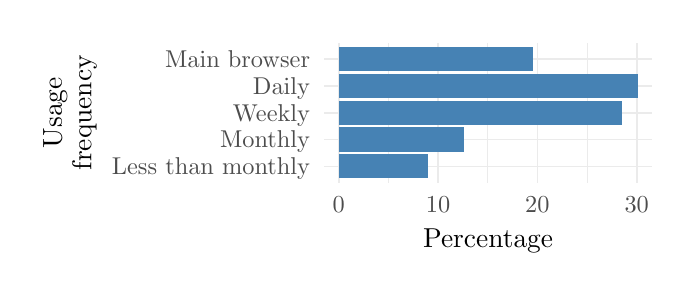
\begin{tikzpicture}[x=1pt,y=1pt]
\definecolor{fillColor}{RGB}{255,255,255}
\path[use as bounding box,fill=fillColor,fill opacity=0.00] (0,0) rectangle (231.26, 86.72);
\begin{scope}
\path[clip] (106.99, 30.77) rectangle (225.76, 81.22);
\definecolor{drawColor}{gray}{0.92}

\path[draw=drawColor,line width= 0.3pt,line join=round] (130.33, 30.77) --
	(130.33, 81.22);

\path[draw=drawColor,line width= 0.3pt,line join=round] (166.23, 30.77) --
	(166.23, 81.22);

\path[draw=drawColor,line width= 0.3pt,line join=round] (202.13, 30.77) --
	(202.13, 81.22);

\path[draw=drawColor,line width= 0.6pt,line join=round] (106.99, 36.59) --
	(225.76, 36.59);

\path[draw=drawColor,line width= 0.6pt,line join=round] (106.99, 46.30) --
	(225.76, 46.30);

\path[draw=drawColor,line width= 0.6pt,line join=round] (106.99, 56.00) --
	(225.76, 56.00);

\path[draw=drawColor,line width= 0.6pt,line join=round] (106.99, 65.70) --
	(225.76, 65.70);

\path[draw=drawColor,line width= 0.6pt,line join=round] (106.99, 75.40) --
	(225.76, 75.40);

\path[draw=drawColor,line width= 0.6pt,line join=round] (112.38, 30.77) --
	(112.38, 81.22);

\path[draw=drawColor,line width= 0.6pt,line join=round] (148.28, 30.77) --
	(148.28, 81.22);

\path[draw=drawColor,line width= 0.6pt,line join=round] (184.18, 30.77) --
	(184.18, 81.22);

\path[draw=drawColor,line width= 0.6pt,line join=round] (220.08, 30.77) --
	(220.08, 81.22);
\definecolor{fillColor}{RGB}{70,130,180}

\path[fill=fillColor] (112.38, 32.23) rectangle (144.69, 40.96);

\path[fill=fillColor] (112.38, 41.93) rectangle (157.76, 50.66);

\path[fill=fillColor] (112.38, 51.63) rectangle (214.84, 60.36);

\path[fill=fillColor] (112.38, 61.33) rectangle (220.36, 70.07);

\path[fill=fillColor] (112.38, 71.04) rectangle (182.53, 79.77);
\end{scope}
\begin{scope}
\path[clip] (  0.00,  0.00) rectangle (231.26, 86.72);
\definecolor{drawColor}{gray}{0.30}

\node[text=drawColor,anchor=base east,inner sep=0pt, outer sep=0pt, scale=  0.88] at (102.04, 33.56) {Less than monthly};

\node[text=drawColor,anchor=base east,inner sep=0pt, outer sep=0pt, scale=  0.88] at (102.04, 43.27) {Monthly};

\node[text=drawColor,anchor=base east,inner sep=0pt, outer sep=0pt, scale=  0.88] at (102.04, 52.97) {Weekly};

\node[text=drawColor,anchor=base east,inner sep=0pt, outer sep=0pt, scale=  0.88] at (102.04, 62.67) {Daily};

\node[text=drawColor,anchor=base east,inner sep=0pt, outer sep=0pt, scale=  0.88] at (102.04, 72.37) {Main browser};
\end{scope}
\begin{scope}
\path[clip] (  0.00,  0.00) rectangle (231.26, 86.72);
\definecolor{drawColor}{gray}{0.30}

\node[text=drawColor,anchor=base,inner sep=0pt, outer sep=0pt, scale=  0.88] at (112.38, 19.76) {0};

\node[text=drawColor,anchor=base,inner sep=0pt, outer sep=0pt, scale=  0.88] at (148.28, 19.76) {10};

\node[text=drawColor,anchor=base,inner sep=0pt, outer sep=0pt, scale=  0.88] at (184.18, 19.76) {20};

\node[text=drawColor,anchor=base,inner sep=0pt, outer sep=0pt, scale=  0.88] at (220.08, 19.76) {30};
\end{scope}
\begin{scope}
\path[clip] (  0.00,  0.00) rectangle (231.26, 86.72);
\definecolor{drawColor}{RGB}{0,0,0}

\node[text=drawColor,anchor=base,inner sep=0pt, outer sep=0pt, scale=  0.99] at (166.37,  7.44) {Percentage};
\end{scope}
\begin{scope}
\path[clip] (  0.00,  0.00) rectangle (231.26, 86.72);
\definecolor{drawColor}{RGB}{0,0,0}

\node[text=drawColor,rotate= 90.00,anchor=base,inner sep=0pt, outer sep=0pt, scale=  0.99] at ( 12.32, 56.00) {Usage};

\node[text=drawColor,rotate= 90.00,anchor=base,inner sep=0pt, outer sep=0pt, scale=  0.99] at ( 23.01, 56.00) {frequency};
\end{scope}
\end{tikzpicture}

    \caption{The usage frequency of Tor Browser among our respondents.  Almost
    half of our respondents use Tor Browser either daily or as their main
    browser.}
    \label{fig:tor-usage}
\end{figure}

\begin{figure}[t]
    \centering
    % Created by tikzDevice version 0.10.1 on 2018-02-09 14:33:04
% !TEX encoding = UTF-8 Unicode
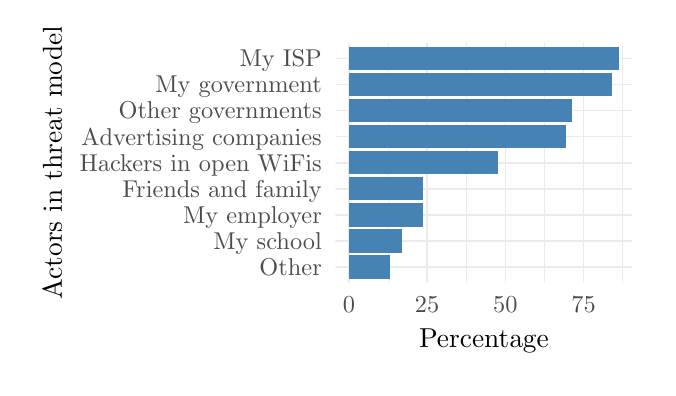
\begin{tikzpicture}[x=1pt,y=1pt]
\definecolor{fillColor}{RGB}{255,255,255}
\path[use as bounding box,fill=fillColor,fill opacity=0.00] (0,0) rectangle (224.04,122.86);
\begin{scope}
\path[clip] (111.23, 30.77) rectangle (218.54,117.36);
\definecolor{drawColor}{gray}{0.92}

\path[draw=drawColor,line width= 0.3pt,line join=round] (130.23, 30.77) --
	(130.23,117.36);

\path[draw=drawColor,line width= 0.3pt,line join=round] (158.48, 30.77) --
	(158.48,117.36);

\path[draw=drawColor,line width= 0.3pt,line join=round] (186.72, 30.77) --
	(186.72,117.36);

\path[draw=drawColor,line width= 0.3pt,line join=round] (214.97, 30.77) --
	(214.97,117.36);

\path[draw=drawColor,line width= 0.6pt,line join=round] (111.23, 36.42) --
	(218.54, 36.42);

\path[draw=drawColor,line width= 0.6pt,line join=round] (111.23, 45.83) --
	(218.54, 45.83);

\path[draw=drawColor,line width= 0.6pt,line join=round] (111.23, 55.24) --
	(218.54, 55.24);

\path[draw=drawColor,line width= 0.6pt,line join=round] (111.23, 64.65) --
	(218.54, 64.65);

\path[draw=drawColor,line width= 0.6pt,line join=round] (111.23, 74.07) --
	(218.54, 74.07);

\path[draw=drawColor,line width= 0.6pt,line join=round] (111.23, 83.48) --
	(218.54, 83.48);

\path[draw=drawColor,line width= 0.6pt,line join=round] (111.23, 92.89) --
	(218.54, 92.89);

\path[draw=drawColor,line width= 0.6pt,line join=round] (111.23,102.30) --
	(218.54,102.30);

\path[draw=drawColor,line width= 0.6pt,line join=round] (111.23,111.71) --
	(218.54,111.71);

\path[draw=drawColor,line width= 0.6pt,line join=round] (116.11, 30.77) --
	(116.11,117.36);

\path[draw=drawColor,line width= 0.6pt,line join=round] (144.35, 30.77) --
	(144.35,117.36);

\path[draw=drawColor,line width= 0.6pt,line join=round] (172.60, 30.77) --
	(172.60,117.36);

\path[draw=drawColor,line width= 0.6pt,line join=round] (200.85, 30.77) --
	(200.85,117.36);
\definecolor{fillColor}{RGB}{70,130,180}

\path[fill=fillColor] (116.11, 32.18) rectangle (130.90, 40.66);

\path[fill=fillColor] (116.11, 41.60) rectangle (135.19, 50.07);

\path[fill=fillColor] (116.11, 51.01) rectangle (142.69, 59.48);

\path[fill=fillColor] (116.11, 60.42) rectangle (142.91, 68.89);

\path[fill=fillColor] (116.11, 69.83) rectangle (169.92, 78.30);

\path[fill=fillColor] (116.11, 79.24) rectangle (194.36, 87.71);

\path[fill=fillColor] (116.11, 88.65) rectangle (196.72, 97.12);

\path[fill=fillColor] (116.11, 98.07) rectangle (211.30,106.54);

\path[fill=fillColor] (116.11,107.48) rectangle (213.66,115.95);
\end{scope}
\begin{scope}
\path[clip] (  0.00,  0.00) rectangle (224.04,122.86);
\definecolor{drawColor}{gray}{0.30}

\node[text=drawColor,anchor=base east,inner sep=0pt, outer sep=0pt, scale=  0.88] at (106.28, 33.39) {Other};

\node[text=drawColor,anchor=base east,inner sep=0pt, outer sep=0pt, scale=  0.88] at (106.28, 42.80) {My school};

\node[text=drawColor,anchor=base east,inner sep=0pt, outer sep=0pt, scale=  0.88] at (106.28, 52.21) {My employer};

\node[text=drawColor,anchor=base east,inner sep=0pt, outer sep=0pt, scale=  0.88] at (106.28, 61.62) {Friends and family};

\node[text=drawColor,anchor=base east,inner sep=0pt, outer sep=0pt, scale=  0.88] at (106.28, 71.04) {Hackers in open WiFis};

\node[text=drawColor,anchor=base east,inner sep=0pt, outer sep=0pt, scale=  0.88] at (106.28, 80.45) {Advertising companies};

\node[text=drawColor,anchor=base east,inner sep=0pt, outer sep=0pt, scale=  0.88] at (106.28, 89.86) {Other governments};

\node[text=drawColor,anchor=base east,inner sep=0pt, outer sep=0pt, scale=  0.88] at (106.28, 99.27) {My government};

\node[text=drawColor,anchor=base east,inner sep=0pt, outer sep=0pt, scale=  0.88] at (106.28,108.68) {My ISP};
\end{scope}
\begin{scope}
\path[clip] (  0.00,  0.00) rectangle (224.04,122.86);
\definecolor{drawColor}{gray}{0.30}

\node[text=drawColor,anchor=base,inner sep=0pt, outer sep=0pt, scale=  0.88] at (116.11, 19.76) {0};

\node[text=drawColor,anchor=base,inner sep=0pt, outer sep=0pt, scale=  0.88] at (144.35, 19.76) {25};

\node[text=drawColor,anchor=base,inner sep=0pt, outer sep=0pt, scale=  0.88] at (172.60, 19.76) {50};

\node[text=drawColor,anchor=base,inner sep=0pt, outer sep=0pt, scale=  0.88] at (200.85, 19.76) {75};
\end{scope}
\begin{scope}
\path[clip] (  0.00,  0.00) rectangle (224.04,122.86);
\definecolor{drawColor}{RGB}{0,0,0}

\node[text=drawColor,anchor=base,inner sep=0pt, outer sep=0pt, scale=  0.99] at (164.88,  7.44) {Percentage};
\end{scope}
\begin{scope}
\path[clip] (  0.00,  0.00) rectangle (224.04,122.86);
\definecolor{drawColor}{RGB}{0,0,0}

\node[text=drawColor,rotate= 90.00,anchor=base,inner sep=0pt, outer sep=0pt, scale=  0.99] at ( 12.32, 74.07) {Actors in threat model};
\end{scope}
\end{tikzpicture}

    \caption{The threat actors that our respondents seek to protect themselves
        from by using Tor Browser.}
    \label{fig:tor-threats}
\end{figure}

People who selected ``Other'' gave a variety of responses.  A number of
respondents specifically pointed out Google and Facebook.  ISPs, backbone ISPs,
and web sites were another common theme.  A number of respondents are struggling
with personal threats that include identity theft, targeted harassment, and
stalking.  Research is another common theme: Several respondents want to learn
about a topic without revealing their interest in it.  Some respondents use Tor
for search engine optimization, computer security research, and to research
medical conditions.  Finally, Tor provides technical advantages that don't
involve a threat actor.  Some respondents want IPv6 connectivity, evasion of
geographical content restrictions, and access to onion services.  A small number
of respondents are only interested in technical aspects other than privacy.  One
respondent stated that they don't need anonymity themselves but instead use Tor
to provide cover traffic for ``people who need protection.''

\subsubsection{Onion service usage}

The usage frequency of onion services is almost uniformly distributed among our
respondents; 24\% use onion sites less than once a month, 22\% use them about
monthly, 25\% weekly, and 23\% daily.  The remaining 6\% has never used an onion
service before.

The majority of our respondents (61.8\%) has used onion services for purposes
other than web browsing before.  Several protocols such as the chat application
Ricochet~\cite{ricochet} and the file sharing application
OnionShare~\cite{onionshare} were purpose-built on top of onion services while
existing TCP-based tools such as SSH can also be used with onion addresses
instead of traditional IP addresses.  Almost one third (29.7\%) of our
participants use onion service for non-browsing activities at least once a week.

But why do Tor users browse onion services in the first place?
Figure~\ref{fig:onion-usage} provides an answer.  The majority uses onion
services because of the additional anonymity (70\%) and the additional security
(61\%).  For 46\% it is the only way to access some content they enjoy, so using
onion services is a necessity.  27\% of our respondents found themselves curious
about the ``Dark Web'' and set out to find their own answer and 19\%
occasionally stumble upon links to onion services in their day-to-day browsing
activity.  Respondents who selected ``Other'' gave a variety of reasons, the
most predominant of which was the ability to set up a TCP service behind a NAT
device.  That way, it is possible to run an SSH server in a home network that
has neither a permanent IP address, nor port forwarding.  Other noteworthy
respondents use onion services to reduce the load on exit relays, to do
technical research, and to access sites that are otherwise unavailable.

\begin{figure}[t]
    \centering
    % Created by tikzDevice version 0.10.1 on 2018-01-12 16:14:57
% !TEX encoding = UTF-8 Unicode
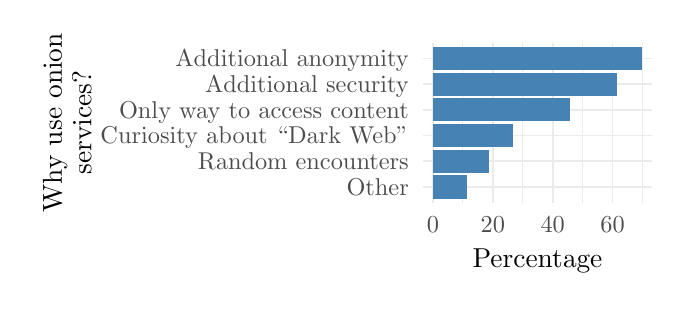
\begin{tikzpicture}[x=1pt,y=1pt]
\definecolor{fillColor}{RGB}{255,255,255}
\path[use as bounding box,fill=fillColor,fill opacity=0.00] (0,0) rectangle (231.26, 93.95);
\begin{scope}
\path[clip] (142.68, 30.77) rectangle (225.76, 88.45);
\definecolor{drawColor}{gray}{0.92}

\path[draw=drawColor,line width= 0.3pt,line join=round] (157.27, 30.77) --
	(157.27, 88.45);

\path[draw=drawColor,line width= 0.3pt,line join=round] (178.90, 30.77) --
	(178.90, 88.45);

\path[draw=drawColor,line width= 0.3pt,line join=round] (200.54, 30.77) --
	(200.54, 88.45);

\path[draw=drawColor,line width= 0.3pt,line join=round] (222.17, 30.77) --
	(222.17, 88.45);

\path[draw=drawColor,line width= 0.6pt,line join=round] (142.68, 36.35) --
	(225.76, 36.35);

\path[draw=drawColor,line width= 0.6pt,line join=round] (142.68, 45.66) --
	(225.76, 45.66);

\path[draw=drawColor,line width= 0.6pt,line join=round] (142.68, 54.96) --
	(225.76, 54.96);

\path[draw=drawColor,line width= 0.6pt,line join=round] (142.68, 64.26) --
	(225.76, 64.26);

\path[draw=drawColor,line width= 0.6pt,line join=round] (142.68, 73.57) --
	(225.76, 73.57);

\path[draw=drawColor,line width= 0.6pt,line join=round] (142.68, 82.87) --
	(225.76, 82.87);

\path[draw=drawColor,line width= 0.6pt,line join=round] (146.45, 30.77) --
	(146.45, 88.45);

\path[draw=drawColor,line width= 0.6pt,line join=round] (168.09, 30.77) --
	(168.09, 88.45);

\path[draw=drawColor,line width= 0.6pt,line join=round] (189.72, 30.77) --
	(189.72, 88.45);

\path[draw=drawColor,line width= 0.6pt,line join=round] (211.35, 30.77) --
	(211.35, 88.45);
\definecolor{fillColor}{RGB}{70,130,180}

\path[fill=fillColor] (146.45, 32.17) rectangle (158.77, 40.54);

\path[fill=fillColor] (146.45, 41.47) rectangle (166.57, 49.84);

\path[fill=fillColor] (146.45, 50.77) rectangle (175.40, 59.15);

\path[fill=fillColor] (146.45, 60.08) rectangle (196.12, 68.45);

\path[fill=fillColor] (146.45, 69.38) rectangle (212.96, 77.75);

\path[fill=fillColor] (146.45, 78.68) rectangle (221.99, 87.06);
\end{scope}
\begin{scope}
\path[clip] (  0.00,  0.00) rectangle (231.26, 93.95);
\definecolor{drawColor}{gray}{0.30}

\node[text=drawColor,anchor=base east,inner sep=0pt, outer sep=0pt, scale=  0.88] at (137.73, 33.32) {Other};

\node[text=drawColor,anchor=base east,inner sep=0pt, outer sep=0pt, scale=  0.88] at (137.73, 42.63) {Random encounters};

\node[text=drawColor,anchor=base east,inner sep=0pt, outer sep=0pt, scale=  0.88] at (137.73, 51.93) {Curiosity about ``Dark Web''};

\node[text=drawColor,anchor=base east,inner sep=0pt, outer sep=0pt, scale=  0.88] at (137.73, 61.23) {Only way to access content};

\node[text=drawColor,anchor=base east,inner sep=0pt, outer sep=0pt, scale=  0.88] at (137.73, 70.54) {Additional security};

\node[text=drawColor,anchor=base east,inner sep=0pt, outer sep=0pt, scale=  0.88] at (137.73, 79.84) {Additional anonymity};
\end{scope}
\begin{scope}
\path[clip] (  0.00,  0.00) rectangle (231.26, 93.95);
\definecolor{drawColor}{gray}{0.30}

\node[text=drawColor,anchor=base,inner sep=0pt, outer sep=0pt, scale=  0.88] at (146.45, 19.76) {0};

\node[text=drawColor,anchor=base,inner sep=0pt, outer sep=0pt, scale=  0.88] at (168.09, 19.76) {20};

\node[text=drawColor,anchor=base,inner sep=0pt, outer sep=0pt, scale=  0.88] at (189.72, 19.76) {40};

\node[text=drawColor,anchor=base,inner sep=0pt, outer sep=0pt, scale=  0.88] at (211.35, 19.76) {60};
\end{scope}
\begin{scope}
\path[clip] (  0.00,  0.00) rectangle (231.26, 93.95);
\definecolor{drawColor}{RGB}{0,0,0}

\node[text=drawColor,anchor=base,inner sep=0pt, outer sep=0pt, scale=  0.99] at (184.22,  7.44) {Percentage};
\end{scope}
\begin{scope}
\path[clip] (  0.00,  0.00) rectangle (231.26, 93.95);
\definecolor{drawColor}{RGB}{0,0,0}

\node[text=drawColor,rotate= 90.00,anchor=base,inner sep=0pt, outer sep=0pt, scale=  0.99] at ( 12.32, 59.61) {Why use onion};

\node[text=drawColor,rotate= 90.00,anchor=base,inner sep=0pt, outer sep=0pt, scale=  0.99] at ( 23.01, 59.61) {services?};
\end{scope}
\end{tikzpicture}

    \caption{Our respondents' (multiple choice) reasons for using onion
    services.}
    \label{fig:onion-usage}
\end{figure}

\subsubsection{Onion service discovery}

Recall that onion services are private by default, leaving it up to their
operator to disseminate the domain.  Established search engines such as Google
are therefore inadequate to find content on onion services.  We wanted to find
out how our respondents discover onion services.
Figure~\ref{fig:onion-discovery} illustrates the results.  The three most
popular ways of discovering new onion sites, all approximating 50\%, are social
networking sites such as Twitter and Reddit, the list of search engines such as
Ahmia\footnote{Ahmia.fi is an onion site search engine that crawls
user-submitted onion domains.  It publishes the list of all indexed onion
services at \url{https://ahmia.fi/onions/}.}, and randomly encountering links
when browsing the web.

While significantly less popular, discovering onion domains through friends and
family has the advantage of trust.  Some of our interview participant indicated
that they heavily rely on this distribution method simply because they can trust
the origin.  Finally, a mere 4\% indicated that they are not interested in
learning about new onion services.

Respondents who selected ``Other'' predominantly brought up
independently-maintained lists of onion services and aggregators.  A noteworthy
example is the Hidden Wiki.

\begin{figure}[t]
    \centering
    % Created by tikzDevice version 0.10.1 on 2018-01-12 16:15:03
% !TEX encoding = UTF-8 Unicode
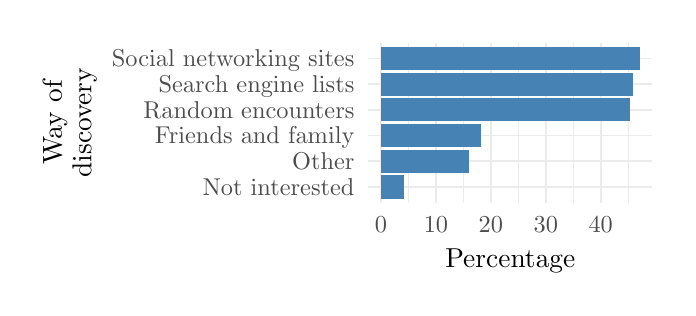
\begin{tikzpicture}[x=1pt,y=1pt]
\definecolor{fillColor}{RGB}{255,255,255}
\path[use as bounding box,fill=fillColor,fill opacity=0.00] (0,0) rectangle (231.26, 93.95);
\begin{scope}
\path[clip] (123.02, 30.77) rectangle (225.76, 88.45);
\definecolor{drawColor}{gray}{0.92}

\path[draw=drawColor,line width= 0.3pt,line join=round] (137.61, 30.77) --
	(137.61, 88.45);

\path[draw=drawColor,line width= 0.3pt,line join=round] (157.46, 30.77) --
	(157.46, 88.45);

\path[draw=drawColor,line width= 0.3pt,line join=round] (177.31, 30.77) --
	(177.31, 88.45);

\path[draw=drawColor,line width= 0.3pt,line join=round] (197.16, 30.77) --
	(197.16, 88.45);

\path[draw=drawColor,line width= 0.3pt,line join=round] (217.00, 30.77) --
	(217.00, 88.45);

\path[draw=drawColor,line width= 0.6pt,line join=round] (123.02, 36.35) --
	(225.76, 36.35);

\path[draw=drawColor,line width= 0.6pt,line join=round] (123.02, 45.66) --
	(225.76, 45.66);

\path[draw=drawColor,line width= 0.6pt,line join=round] (123.02, 54.96) --
	(225.76, 54.96);

\path[draw=drawColor,line width= 0.6pt,line join=round] (123.02, 64.26) --
	(225.76, 64.26);

\path[draw=drawColor,line width= 0.6pt,line join=round] (123.02, 73.57) --
	(225.76, 73.57);

\path[draw=drawColor,line width= 0.6pt,line join=round] (123.02, 82.87) --
	(225.76, 82.87);

\path[draw=drawColor,line width= 0.6pt,line join=round] (127.69, 30.77) --
	(127.69, 88.45);

\path[draw=drawColor,line width= 0.6pt,line join=round] (147.54, 30.77) --
	(147.54, 88.45);

\path[draw=drawColor,line width= 0.6pt,line join=round] (167.38, 30.77) --
	(167.38, 88.45);

\path[draw=drawColor,line width= 0.6pt,line join=round] (187.23, 30.77) --
	(187.23, 88.45);

\path[draw=drawColor,line width= 0.6pt,line join=round] (207.08, 30.77) --
	(207.08, 88.45);
\definecolor{fillColor}{RGB}{70,130,180}

\path[fill=fillColor] (127.69, 32.17) rectangle (135.96, 40.54);

\path[fill=fillColor] (127.69, 41.47) rectangle (159.33, 49.84);

\path[fill=fillColor] (127.69, 50.77) rectangle (163.85, 59.15);

\path[fill=fillColor] (127.69, 60.08) rectangle (217.70, 68.45);

\path[fill=fillColor] (127.69, 69.38) rectangle (218.83, 77.75);

\path[fill=fillColor] (127.69, 78.68) rectangle (221.09, 87.06);
\end{scope}
\begin{scope}
\path[clip] (  0.00,  0.00) rectangle (231.26, 93.95);
\definecolor{drawColor}{gray}{0.30}

\node[text=drawColor,anchor=base east,inner sep=0pt, outer sep=0pt, scale=  0.88] at (118.07, 33.32) {Not interested};

\node[text=drawColor,anchor=base east,inner sep=0pt, outer sep=0pt, scale=  0.88] at (118.07, 42.63) {Other};

\node[text=drawColor,anchor=base east,inner sep=0pt, outer sep=0pt, scale=  0.88] at (118.07, 51.93) {Friends and family};

\node[text=drawColor,anchor=base east,inner sep=0pt, outer sep=0pt, scale=  0.88] at (118.07, 61.23) {Random encounters};

\node[text=drawColor,anchor=base east,inner sep=0pt, outer sep=0pt, scale=  0.88] at (118.07, 70.54) {Search engine lists};

\node[text=drawColor,anchor=base east,inner sep=0pt, outer sep=0pt, scale=  0.88] at (118.07, 79.84) {Social networking sites};
\end{scope}
\begin{scope}
\path[clip] (  0.00,  0.00) rectangle (231.26, 93.95);
\definecolor{drawColor}{gray}{0.30}

\node[text=drawColor,anchor=base,inner sep=0pt, outer sep=0pt, scale=  0.88] at (127.69, 19.76) {0};

\node[text=drawColor,anchor=base,inner sep=0pt, outer sep=0pt, scale=  0.88] at (147.54, 19.76) {10};

\node[text=drawColor,anchor=base,inner sep=0pt, outer sep=0pt, scale=  0.88] at (167.38, 19.76) {20};

\node[text=drawColor,anchor=base,inner sep=0pt, outer sep=0pt, scale=  0.88] at (187.23, 19.76) {30};

\node[text=drawColor,anchor=base,inner sep=0pt, outer sep=0pt, scale=  0.88] at (207.08, 19.76) {40};
\end{scope}
\begin{scope}
\path[clip] (  0.00,  0.00) rectangle (231.26, 93.95);
\definecolor{drawColor}{RGB}{0,0,0}

\node[text=drawColor,anchor=base,inner sep=0pt, outer sep=0pt, scale=  0.99] at (174.39,  7.44) {Percentage};
\end{scope}
\begin{scope}
\path[clip] (  0.00,  0.00) rectangle (231.26, 93.95);
\definecolor{drawColor}{RGB}{0,0,0}

\node[text=drawColor,rotate= 90.00,anchor=base,inner sep=0pt, outer sep=0pt, scale=  0.99] at ( 12.32, 59.61) {Way of};

\node[text=drawColor,rotate= 90.00,anchor=base,inner sep=0pt, outer sep=0pt, scale=  0.99] at ( 23.01, 59.61) {discovery};
\end{scope}
\end{tikzpicture}

    \caption{Our respondents' (multiple choice) methods of discovering onion
    services.}
    \label{fig:onion-discovery}
\end{figure}

The next question in our survey then asked if our respondents are satisfied with
the way they discover onion services.  60\% selected ``Yes'' while 40\% selected
``No.'' Some respondents who selected ``Yes'' brought up that they have no
interest in learning about new onion services, in part because they only use a
small set of onion services.  Among the people who are not satisfied, the most
prominent complaint was about broken links on onion site lists.  There is
non-trivial churn among onion sites and our respondents were frustrated that
existing lists are typically not curated and contain many dead links.

Many respondents were not aware of search engines such as ahmia.fi.  Among those
that were, many were not satisfied with both the search results and the number
of indexed onion sites.  Unsurprisingly, a ``Google for onion sites'' was a
frequent wish.

Several respondents were unhappy with existing aggregators.  In addition to
broken links, some distrust lists because they occasionally contain scam and
phishing sites.  The difficulty of telling apart two given onion domain names
exacerbates this issue.  Another common wish for aggregators was for them to be
more verbose in their description of onion sites.  In particular, some
respondents want to avoid illegal and pornographic content, which is often
difficult if the description is vague and the onion domain reveals nothing about
its content.

Many respondents expressed frustration about the difficulty of finding out if
site X also provides a corresponding onion service.  A common wish was to have
site X list its onion service prominently in a footer.  Ironically, some
respondents were surprised that torproject.org has a corresponding onion site --
they couldn't find it on the web site.

Interestingly, some respondents voiced frustration about various usability
issues, but mentioned in the same sentence that this is an inherent trade-off of
privacy technology, suggesting that there is nothing that can be done about it.

\subsubsection{Onion service domain format}

Conventional domains are designed to be easy to remember and recognize.  But how do users
handle the randomly-generated onion domains?  Question 3.8 in our survey asked
exactly that, with the responses being illustrated in
Figure~\ref{fig:onion-domain-mgmt}.

\begin{figure}[t]
    \centering
    % Created by tikzDevice version 0.10.1 on 2018-02-09 14:36:33
% !TEX encoding = UTF-8 Unicode
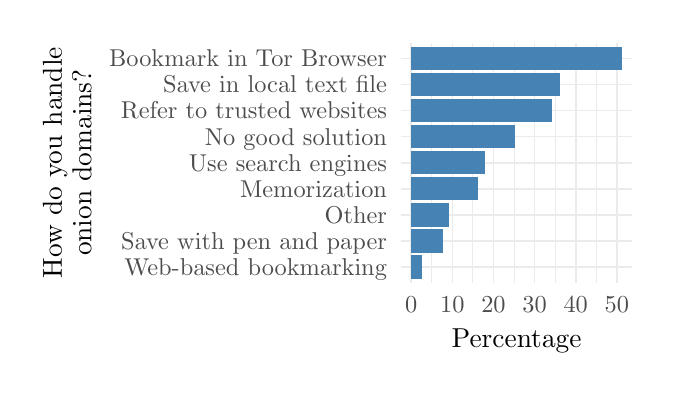
\begin{tikzpicture}[x=1pt,y=1pt]
\definecolor{fillColor}{RGB}{255,255,255}
\path[use as bounding box,fill=fillColor,fill opacity=0.00] (0,0) rectangle (224.04,122.86);
\begin{scope}
\path[clip] (134.78, 30.77) rectangle (218.54,117.36);
\definecolor{drawColor}{gray}{0.92}

\path[draw=drawColor,line width= 0.3pt,line join=round] (146.02, 30.77) --
	(146.02,117.36);

\path[draw=drawColor,line width= 0.3pt,line join=round] (160.88, 30.77) --
	(160.88,117.36);

\path[draw=drawColor,line width= 0.3pt,line join=round] (175.74, 30.77) --
	(175.74,117.36);

\path[draw=drawColor,line width= 0.3pt,line join=round] (190.61, 30.77) --
	(190.61,117.36);

\path[draw=drawColor,line width= 0.3pt,line join=round] (205.47, 30.77) --
	(205.47,117.36);

\path[draw=drawColor,line width= 0.6pt,line join=round] (134.78, 36.42) --
	(218.54, 36.42);

\path[draw=drawColor,line width= 0.6pt,line join=round] (134.78, 45.83) --
	(218.54, 45.83);

\path[draw=drawColor,line width= 0.6pt,line join=round] (134.78, 55.24) --
	(218.54, 55.24);

\path[draw=drawColor,line width= 0.6pt,line join=round] (134.78, 64.65) --
	(218.54, 64.65);

\path[draw=drawColor,line width= 0.6pt,line join=round] (134.78, 74.07) --
	(218.54, 74.07);

\path[draw=drawColor,line width= 0.6pt,line join=round] (134.78, 83.48) --
	(218.54, 83.48);

\path[draw=drawColor,line width= 0.6pt,line join=round] (134.78, 92.89) --
	(218.54, 92.89);

\path[draw=drawColor,line width= 0.6pt,line join=round] (134.78,102.30) --
	(218.54,102.30);

\path[draw=drawColor,line width= 0.6pt,line join=round] (134.78,111.71) --
	(218.54,111.71);

\path[draw=drawColor,line width= 0.6pt,line join=round] (138.58, 30.77) --
	(138.58,117.36);

\path[draw=drawColor,line width= 0.6pt,line join=round] (153.45, 30.77) --
	(153.45,117.36);

\path[draw=drawColor,line width= 0.6pt,line join=round] (168.31, 30.77) --
	(168.31,117.36);

\path[draw=drawColor,line width= 0.6pt,line join=round] (183.17, 30.77) --
	(183.17,117.36);

\path[draw=drawColor,line width= 0.6pt,line join=round] (198.04, 30.77) --
	(198.04,117.36);

\path[draw=drawColor,line width= 0.6pt,line join=round] (212.90, 30.77) --
	(212.90,117.36);
\definecolor{fillColor}{RGB}{70,130,180}

\path[fill=fillColor] (138.58, 32.18) rectangle (142.54, 40.66);

\path[fill=fillColor] (138.58, 41.60) rectangle (150.15, 50.07);

\path[fill=fillColor] (138.58, 51.01) rectangle (152.13, 59.48);

\path[fill=fillColor] (138.58, 60.42) rectangle (162.84, 68.89);

\path[fill=fillColor] (138.58, 69.83) rectangle (165.10, 78.30);

\path[fill=fillColor] (138.58, 79.24) rectangle (176.10, 87.71);

\path[fill=fillColor] (138.58, 88.65) rectangle (189.36, 97.12);

\path[fill=fillColor] (138.58, 98.07) rectangle (192.45,106.54);

\path[fill=fillColor] (138.58,107.48) rectangle (214.73,115.95);
\end{scope}
\begin{scope}
\path[clip] (  0.00,  0.00) rectangle (224.04,122.86);
\definecolor{drawColor}{gray}{0.30}

\node[text=drawColor,anchor=base east,inner sep=0pt, outer sep=0pt, scale=  0.88] at (129.83, 33.39) {Web-based bookmarking};

\node[text=drawColor,anchor=base east,inner sep=0pt, outer sep=0pt, scale=  0.88] at (129.83, 42.80) {Save with pen and paper};

\node[text=drawColor,anchor=base east,inner sep=0pt, outer sep=0pt, scale=  0.88] at (129.83, 52.21) {Other};

\node[text=drawColor,anchor=base east,inner sep=0pt, outer sep=0pt, scale=  0.88] at (129.83, 61.62) {Memorization};

\node[text=drawColor,anchor=base east,inner sep=0pt, outer sep=0pt, scale=  0.88] at (129.83, 71.04) {Use search engines};

\node[text=drawColor,anchor=base east,inner sep=0pt, outer sep=0pt, scale=  0.88] at (129.83, 80.45) {No good solution};

\node[text=drawColor,anchor=base east,inner sep=0pt, outer sep=0pt, scale=  0.88] at (129.83, 89.86) {Refer to trusted websites};

\node[text=drawColor,anchor=base east,inner sep=0pt, outer sep=0pt, scale=  0.88] at (129.83, 99.27) {Save in local text file};

\node[text=drawColor,anchor=base east,inner sep=0pt, outer sep=0pt, scale=  0.88] at (129.83,108.68) {Bookmark in Tor Browser};
\end{scope}
\begin{scope}
\path[clip] (  0.00,  0.00) rectangle (224.04,122.86);
\definecolor{drawColor}{gray}{0.30}

\node[text=drawColor,anchor=base,inner sep=0pt, outer sep=0pt, scale=  0.88] at (138.58, 19.76) {0};

\node[text=drawColor,anchor=base,inner sep=0pt, outer sep=0pt, scale=  0.88] at (153.45, 19.76) {10};

\node[text=drawColor,anchor=base,inner sep=0pt, outer sep=0pt, scale=  0.88] at (168.31, 19.76) {20};

\node[text=drawColor,anchor=base,inner sep=0pt, outer sep=0pt, scale=  0.88] at (183.17, 19.76) {30};

\node[text=drawColor,anchor=base,inner sep=0pt, outer sep=0pt, scale=  0.88] at (198.04, 19.76) {40};

\node[text=drawColor,anchor=base,inner sep=0pt, outer sep=0pt, scale=  0.88] at (212.90, 19.76) {50};
\end{scope}
\begin{scope}
\path[clip] (  0.00,  0.00) rectangle (224.04,122.86);
\definecolor{drawColor}{RGB}{0,0,0}

\node[text=drawColor,anchor=base,inner sep=0pt, outer sep=0pt, scale=  0.99] at (176.66,  7.44) {Percentage};
\end{scope}
\begin{scope}
\path[clip] (  0.00,  0.00) rectangle (224.04,122.86);
\definecolor{drawColor}{RGB}{0,0,0}

\node[text=drawColor,rotate= 90.00,anchor=base,inner sep=0pt, outer sep=0pt, scale=  0.99] at ( 12.32, 74.07) {How do you handle};

\node[text=drawColor,rotate= 90.00,anchor=base,inner sep=0pt, outer sep=0pt, scale=  0.99] at ( 23.01, 74.07) {onion domains?};
\end{scope}
\end{tikzpicture}

    \caption{The strategies that our respondents use to handle onion domains.
    More than half use bookmarks inside of Tor Browser and a quarter thinks that
    there's no good solution.}
    \label{fig:onion-domain-mgmt}
\end{figure}

Most respondents use bookmarks inside Tor Browser for onion domains.  While
convenient, it leaves a trace of (presumably) visited sites on one's computer.
One of Tor Browser's security requirements is ``disk avoidance,'' \ie, the
browser must not write anything to disk that would reveal the user's browsing
history~\cite[\S~2.1]{Perry2017a}.  Bookmarking links is a violation of this
security requirement.  Many of our respondents were aware of this issue.  About
a dozen respondents who selected ``Other'' stated that they store onion domains
encryptedly---either in a text file or in their password manager.

Somewhat less popular is saving onion domains in local text files (36\%),
getting them from trusted web sites (34\%), use search engines (18\%), memorize
domains (16\%), use some other techniques (9\%) or employ pen and paper (8\%).
Notably, one quarter of our respondents does not have a good solution to the
problem.  Given the alarming number of (possibly insecure) home-baked solutions,
a Tor Browser extension may be warranted to approach the problem.

The next question in our survey asked if our respondents expect the
next-generation domain format to change their browsing habits.  Interestingly,
only 17\% expect to have their browsing habits changed while 83\% don't.  Among
the respondents who selected ``Yes,'' many expressed that they memorize a small
number of onion domains (such as Facebook's), which will no longer be possible.
People who selected ``No'' mostly bring up that they treat onion domains as
opaque identifiers that they handle via tools such as bookmarks.  These results
suggest that the current state is dire, yet not expected to get much worse with
the new domain format.

Problematic:
``I only memorize the first part of the domain''

``If there isn't some cognizable word at the start, it'll be more difficult for
me to determine if I'm going to the correct domain or a scam. I may end up going
to less .onion sites as a result.''

\subsubsection{Onion service operation}

A survey question block on onion service operation shed light on the reasons for
running onion services and what sort of issues users face when doing so.  40\%
of our respondents once set up an onion service.  Among the respondents who
never have, 31\% have considered doing so while 30\% have never even considered
it.  Interestingly, 79\% of operators have run an onion service for private use
while 53\% have run them for the public.

Figure~\ref{fig:onion-operation-reasons} gives an overview of the reasons for
running onion services.  Interestingly, the extra security properties overshadow
the anonymity properties of onion services.  Another particularly popular reason
is NAT traversal---many respondents noted that onion services allow them to
expose a TCP service in their home network despite being behind a NAT device.
Finally, some people run onion service indirectly because third-party tools such
as OnionShare~\cite{onionshare} or Ricochet~\cite{ricochet} are built on top of
them.  Onion services can have clear benefits for businesses as well as
evidenced by one respondent who wrote on onion services: ``We use it for
delivering updates to our router to customers securely and without leaking
metadata.''

\begin{figure}[t]
    \centering
    % Created by tikzDevice version 0.10.1 on 2018-01-12 16:24:46
% !TEX encoding = UTF-8 Unicode
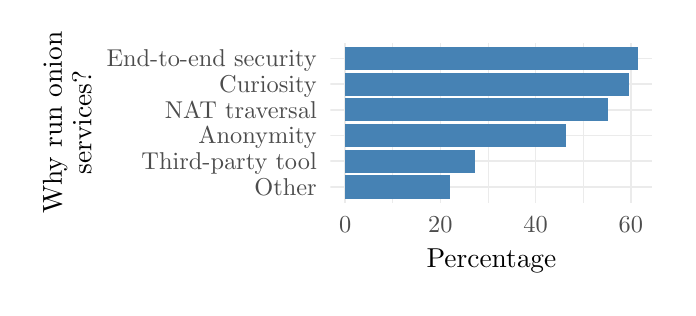
\begin{tikzpicture}[x=1pt,y=1pt]
\definecolor{fillColor}{RGB}{255,255,255}
\path[use as bounding box,fill=fillColor,fill opacity=0.00] (0,0) rectangle (231.26, 93.95);
\begin{scope}
\path[clip] (109.42, 30.77) rectangle (225.76, 88.45);
\definecolor{drawColor}{gray}{0.92}

\path[draw=drawColor,line width= 0.3pt,line join=round] (131.91, 30.77) --
	(131.91, 88.45);

\path[draw=drawColor,line width= 0.3pt,line join=round] (166.33, 30.77) --
	(166.33, 88.45);

\path[draw=drawColor,line width= 0.3pt,line join=round] (200.75, 30.77) --
	(200.75, 88.45);

\path[draw=drawColor,line width= 0.6pt,line join=round] (109.42, 36.35) --
	(225.76, 36.35);

\path[draw=drawColor,line width= 0.6pt,line join=round] (109.42, 45.66) --
	(225.76, 45.66);

\path[draw=drawColor,line width= 0.6pt,line join=round] (109.42, 54.96) --
	(225.76, 54.96);

\path[draw=drawColor,line width= 0.6pt,line join=round] (109.42, 64.26) --
	(225.76, 64.26);

\path[draw=drawColor,line width= 0.6pt,line join=round] (109.42, 73.57) --
	(225.76, 73.57);

\path[draw=drawColor,line width= 0.6pt,line join=round] (109.42, 82.87) --
	(225.76, 82.87);

\path[draw=drawColor,line width= 0.6pt,line join=round] (114.70, 30.77) --
	(114.70, 88.45);

\path[draw=drawColor,line width= 0.6pt,line join=round] (149.12, 30.77) --
	(149.12, 88.45);

\path[draw=drawColor,line width= 0.6pt,line join=round] (183.54, 30.77) --
	(183.54, 88.45);

\path[draw=drawColor,line width= 0.6pt,line join=round] (217.96, 30.77) --
	(217.96, 88.45);
\definecolor{fillColor}{RGB}{70,130,180}

\path[fill=fillColor] (114.70, 32.17) rectangle (152.48, 40.54);

\path[fill=fillColor] (114.70, 41.47) rectangle (161.72, 49.84);

\path[fill=fillColor] (114.70, 50.77) rectangle (194.45, 59.15);

\path[fill=fillColor] (114.70, 60.08) rectangle (209.56, 68.45);

\path[fill=fillColor] (114.70, 69.38) rectangle (217.12, 77.75);

\path[fill=fillColor] (114.70, 78.68) rectangle (220.48, 87.06);
\end{scope}
\begin{scope}
\path[clip] (  0.00,  0.00) rectangle (231.26, 93.95);
\definecolor{drawColor}{gray}{0.30}

\node[text=drawColor,anchor=base east,inner sep=0pt, outer sep=0pt, scale=  0.88] at (104.47, 33.32) {Other};

\node[text=drawColor,anchor=base east,inner sep=0pt, outer sep=0pt, scale=  0.88] at (104.47, 42.63) {Third-party tool};

\node[text=drawColor,anchor=base east,inner sep=0pt, outer sep=0pt, scale=  0.88] at (104.47, 51.93) {Anonymity};

\node[text=drawColor,anchor=base east,inner sep=0pt, outer sep=0pt, scale=  0.88] at (104.47, 61.23) {NAT traversal};

\node[text=drawColor,anchor=base east,inner sep=0pt, outer sep=0pt, scale=  0.88] at (104.47, 70.54) {Curiosity};

\node[text=drawColor,anchor=base east,inner sep=0pt, outer sep=0pt, scale=  0.88] at (104.47, 79.84) {End-to-end security};
\end{scope}
\begin{scope}
\path[clip] (  0.00,  0.00) rectangle (231.26, 93.95);
\definecolor{drawColor}{gray}{0.30}

\node[text=drawColor,anchor=base,inner sep=0pt, outer sep=0pt, scale=  0.88] at (114.70, 19.76) {0};

\node[text=drawColor,anchor=base,inner sep=0pt, outer sep=0pt, scale=  0.88] at (149.12, 19.76) {20};

\node[text=drawColor,anchor=base,inner sep=0pt, outer sep=0pt, scale=  0.88] at (183.54, 19.76) {40};

\node[text=drawColor,anchor=base,inner sep=0pt, outer sep=0pt, scale=  0.88] at (217.96, 19.76) {60};
\end{scope}
\begin{scope}
\path[clip] (  0.00,  0.00) rectangle (231.26, 93.95);
\definecolor{drawColor}{RGB}{0,0,0}

\node[text=drawColor,anchor=base,inner sep=0pt, outer sep=0pt, scale=  0.99] at (167.59,  7.44) {Percentage};
\end{scope}
\begin{scope}
\path[clip] (  0.00,  0.00) rectangle (231.26, 93.95);
\definecolor{drawColor}{RGB}{0,0,0}

\node[text=drawColor,rotate= 90.00,anchor=base,inner sep=0pt, outer sep=0pt, scale=  0.99] at ( 12.32, 59.61) {Why run onion};

\node[text=drawColor,rotate= 90.00,anchor=base,inner sep=0pt, outer sep=0pt, scale=  0.99] at ( 23.01, 59.61) {services?};
\end{scope}
\end{tikzpicture}

    \caption{The reasons people have for running onion services.}
    \label{fig:onion-operation-reasons}
\end{figure}

Figure~\ref{fig:onion-operation-concerns} illustrates the concerns that onion
service operators face.  We consider three attacks; \first somebody setting up a
phishing site for the operator's site, \second a denial-of-service attack, and
\third a deanonymization attack.  More than half of our respondents are at least
somewhat concerned about all of these attacks.  Almost 40\% claim to be
extremely concerned about somebody deanonymizing their onion service.  Indeed,
many respondents lamented the difficulty of knowing that an onion service setup
is robust against application-layer deanonymization attacks.

\begin{figure}[t]
    \centering
    % Created by tikzDevice version 0.10.1 on 2018-02-09 14:59:34
% !TEX encoding = UTF-8 Unicode
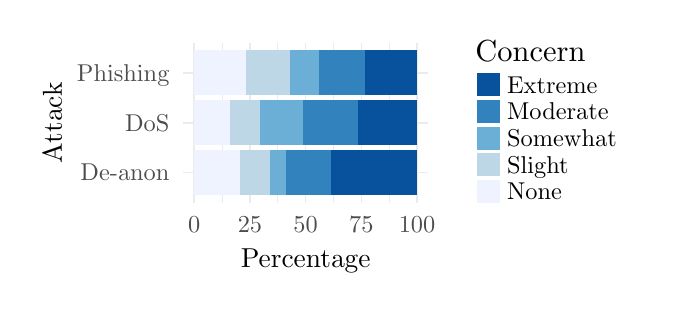
\begin{tikzpicture}[x=1pt,y=1pt]
\definecolor{fillColor}{RGB}{255,255,255}
\path[use as bounding box,fill=fillColor,fill opacity=0.00] (0,0) rectangle (224.04, 93.95);
\begin{scope}
\path[clip] ( 56.18, 30.77) rectangle (144.74, 88.45);
\definecolor{drawColor}{gray}{0.92}

\path[draw=drawColor,line width= 0.3pt,line join=round] ( 70.26, 30.77) --
	( 70.26, 88.45);

\path[draw=drawColor,line width= 0.3pt,line join=round] ( 90.39, 30.77) --
	( 90.39, 88.45);

\path[draw=drawColor,line width= 0.3pt,line join=round] (110.52, 30.77) --
	(110.52, 88.45);

\path[draw=drawColor,line width= 0.3pt,line join=round] (130.64, 30.77) --
	(130.64, 88.45);

\path[draw=drawColor,line width= 0.6pt,line join=round] ( 56.18, 41.59) --
	(144.74, 41.59);

\path[draw=drawColor,line width= 0.6pt,line join=round] ( 56.18, 59.61) --
	(144.74, 59.61);

\path[draw=drawColor,line width= 0.6pt,line join=round] ( 56.18, 77.64) --
	(144.74, 77.64);

\path[draw=drawColor,line width= 0.6pt,line join=round] ( 60.20, 30.77) --
	( 60.20, 88.45);

\path[draw=drawColor,line width= 0.6pt,line join=round] ( 80.33, 30.77) --
	( 80.33, 88.45);

\path[draw=drawColor,line width= 0.6pt,line join=round] (100.45, 30.77) --
	(100.45, 88.45);

\path[draw=drawColor,line width= 0.6pt,line join=round] (120.58, 30.77) --
	(120.58, 88.45);

\path[draw=drawColor,line width= 0.6pt,line join=round] (140.71, 30.77) --
	(140.71, 88.45);
\definecolor{fillColor}{RGB}{239,243,255}

\path[fill=fillColor] ( 60.20, 33.48) rectangle ( 76.78, 49.70);
\definecolor{fillColor}{RGB}{189,215,231}

\path[fill=fillColor] ( 76.78, 33.48) rectangle ( 87.44, 49.70);
\definecolor{fillColor}{RGB}{107,174,214}

\path[fill=fillColor] ( 87.44, 33.48) rectangle ( 93.35, 49.70);
\definecolor{fillColor}{RGB}{49,130,189}

\path[fill=fillColor] ( 93.35, 33.48) rectangle (109.54, 49.70);
\definecolor{fillColor}{RGB}{8,81,156}

\path[fill=fillColor] (109.54, 33.48) rectangle (140.72, 49.70);
\definecolor{fillColor}{RGB}{239,243,255}

\path[fill=fillColor] ( 60.20, 51.50) rectangle ( 73.16, 67.72);
\definecolor{fillColor}{RGB}{189,215,231}

\path[fill=fillColor] ( 73.16, 51.50) rectangle ( 83.77, 67.72);
\definecolor{fillColor}{RGB}{107,174,214}

\path[fill=fillColor] ( 83.77, 51.50) rectangle ( 99.47, 67.72);
\definecolor{fillColor}{RGB}{49,130,189}

\path[fill=fillColor] ( 99.47, 51.50) rectangle (119.50, 67.72);
\definecolor{fillColor}{RGB}{8,81,156}

\path[fill=fillColor] (119.50, 51.50) rectangle (140.71, 67.72);
\definecolor{fillColor}{RGB}{239,243,255}

\path[fill=fillColor] ( 60.20, 69.53) rectangle ( 79.05, 85.75);
\definecolor{fillColor}{RGB}{189,215,231}

\path[fill=fillColor] ( 79.05, 69.53) rectangle ( 94.75, 85.75);
\definecolor{fillColor}{RGB}{107,174,214}

\path[fill=fillColor] ( 94.75, 69.53) rectangle (105.36, 85.75);
\definecolor{fillColor}{RGB}{49,130,189}

\path[fill=fillColor] (105.36, 69.53) rectangle (121.85, 85.75);
\definecolor{fillColor}{RGB}{8,81,156}

\path[fill=fillColor] (121.85, 69.53) rectangle (140.70, 85.75);
\end{scope}
\begin{scope}
\path[clip] (  0.00,  0.00) rectangle (224.04, 93.95);
\definecolor{drawColor}{gray}{0.30}

\node[text=drawColor,anchor=base east,inner sep=0pt, outer sep=0pt, scale=  0.88] at ( 51.23, 38.56) {De-anon};

\node[text=drawColor,anchor=base east,inner sep=0pt, outer sep=0pt, scale=  0.88] at ( 51.23, 56.58) {DoS};

\node[text=drawColor,anchor=base east,inner sep=0pt, outer sep=0pt, scale=  0.88] at ( 51.23, 74.61) {Phishing};
\end{scope}
\begin{scope}
\path[clip] (  0.00,  0.00) rectangle (224.04, 93.95);
\definecolor{drawColor}{gray}{0.30}

\node[text=drawColor,anchor=base,inner sep=0pt, outer sep=0pt, scale=  0.88] at ( 60.20, 19.76) {0};

\node[text=drawColor,anchor=base,inner sep=0pt, outer sep=0pt, scale=  0.88] at ( 80.33, 19.76) {25};

\node[text=drawColor,anchor=base,inner sep=0pt, outer sep=0pt, scale=  0.88] at (100.45, 19.76) {50};

\node[text=drawColor,anchor=base,inner sep=0pt, outer sep=0pt, scale=  0.88] at (120.58, 19.76) {75};

\node[text=drawColor,anchor=base,inner sep=0pt, outer sep=0pt, scale=  0.88] at (140.71, 19.76) {100};
\end{scope}
\begin{scope}
\path[clip] (  0.00,  0.00) rectangle (224.04, 93.95);
\definecolor{drawColor}{RGB}{0,0,0}

\node[text=drawColor,anchor=base,inner sep=0pt, outer sep=0pt, scale=  0.99] at (100.46,  7.44) {Percentage};
\end{scope}
\begin{scope}
\path[clip] (  0.00,  0.00) rectangle (224.04, 93.95);
\definecolor{drawColor}{RGB}{0,0,0}

\node[text=drawColor,rotate= 90.00,anchor=base,inner sep=0pt, outer sep=0pt, scale=  0.99] at ( 12.32, 59.61) {Attack};
\end{scope}
\begin{scope}
\path[clip] (  0.00,  0.00) rectangle (224.04, 93.95);
\definecolor{drawColor}{RGB}{0,0,0}

\node[text=drawColor,anchor=base west,inner sep=0pt, outer sep=0pt, scale=  1.10] at (161.81, 81.72) {Concern};
\end{scope}
\begin{scope}
\path[clip] (  0.00,  0.00) rectangle (224.04, 93.95);
\definecolor{fillColor}{RGB}{8,81,156}

\path[fill=fillColor] (162.52, 69.18) rectangle (170.74, 77.40);
\end{scope}
\begin{scope}
\path[clip] (  0.00,  0.00) rectangle (224.04, 93.95);
\definecolor{fillColor}{RGB}{49,130,189}

\path[fill=fillColor] (162.52, 59.55) rectangle (170.74, 67.76);
\end{scope}
\begin{scope}
\path[clip] (  0.00,  0.00) rectangle (224.04, 93.95);
\definecolor{fillColor}{RGB}{107,174,214}

\path[fill=fillColor] (162.52, 49.91) rectangle (170.74, 58.12);
\end{scope}
\begin{scope}
\path[clip] (  0.00,  0.00) rectangle (224.04, 93.95);
\definecolor{fillColor}{RGB}{189,215,231}

\path[fill=fillColor] (162.52, 40.27) rectangle (170.74, 48.49);
\end{scope}
\begin{scope}
\path[clip] (  0.00,  0.00) rectangle (224.04, 93.95);
\definecolor{fillColor}{RGB}{239,243,255}

\path[fill=fillColor] (162.52, 30.64) rectangle (170.74, 38.85);
\end{scope}
\begin{scope}
\path[clip] (  0.00,  0.00) rectangle (224.04, 93.95);
\definecolor{drawColor}{RGB}{0,0,0}

\node[text=drawColor,anchor=base west,inner sep=0pt, outer sep=0pt, scale=  0.88] at (173.26, 70.26) {Extreme};
\end{scope}
\begin{scope}
\path[clip] (  0.00,  0.00) rectangle (224.04, 93.95);
\definecolor{drawColor}{RGB}{0,0,0}

\node[text=drawColor,anchor=base west,inner sep=0pt, outer sep=0pt, scale=  0.88] at (173.26, 60.62) {Moderate};
\end{scope}
\begin{scope}
\path[clip] (  0.00,  0.00) rectangle (224.04, 93.95);
\definecolor{drawColor}{RGB}{0,0,0}

\node[text=drawColor,anchor=base west,inner sep=0pt, outer sep=0pt, scale=  0.88] at (173.26, 50.99) {Somewhat};
\end{scope}
\begin{scope}
\path[clip] (  0.00,  0.00) rectangle (224.04, 93.95);
\definecolor{drawColor}{RGB}{0,0,0}

\node[text=drawColor,anchor=base west,inner sep=0pt, outer sep=0pt, scale=  0.88] at (173.26, 41.35) {Slight};
\end{scope}
\begin{scope}
\path[clip] (  0.00,  0.00) rectangle (224.04, 93.95);
\definecolor{drawColor}{RGB}{0,0,0}

\node[text=drawColor,anchor=base west,inner sep=0pt, outer sep=0pt, scale=  0.88] at (173.26, 31.71) {None};
\end{scope}
\end{tikzpicture}

    \caption{The level of concern onion service operators have with respect to a
    phishing clone of their service, denial-of-service attacks, and
    deanonymization.}
    \label{fig:onion-operation-concerns}
\end{figure}

\subsubsection{Susceptibility to phishing attacks}

Phishing remains an issue despite onion services' extra anonymity and security
properties.  Past work has uncovered an attack that transparently rewrote
Bitcoin addresses to hijack Bitcoin
transactions~\cite{Winter2016a,Nurmi2015a,Monteiro2016a}.  Key to this attack is
the difficulty of telling apart an authentic from an impersonation domain.  For
conventional domains we rely on (EV) certificates, browser protections, search
results, and long-lived reputation, but none of these methods work well for
onion services.  Does the nature of onion services facilitate phishing attacks?
If so, what can we do to mitigate the issue?

We asked our respondents if they ever thought about the authenticity of an onion
site.  With 80\%, the majority of our respondents did while 20\% didn't.
Clearly, there is a need for verification but how does one verify that an onion
service is authentic?  Figure~\ref{fig:determining-legitimacy} gives an overview
of the strategies that our respondents employ.

\begin{figure}[t]
    \centering
    % Created by tikzDevice version 0.10.1 on 2018-01-12 16:30:02
% !TEX encoding = UTF-8 Unicode
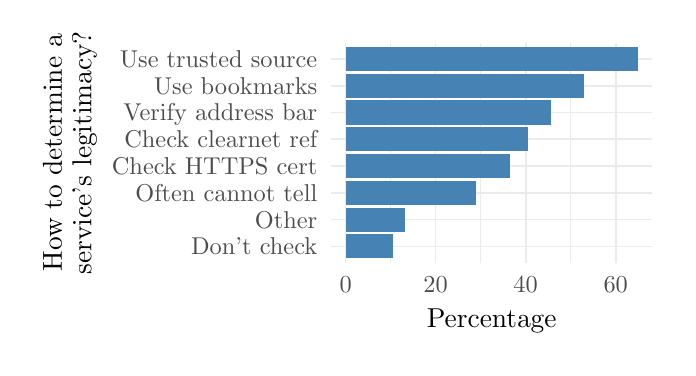
\begin{tikzpicture}[x=1pt,y=1pt]
\definecolor{fillColor}{RGB}{255,255,255}
\path[use as bounding box,fill=fillColor,fill opacity=0.00] (0,0) rectangle (231.26,115.63);
\begin{scope}
\path[clip] (109.60, 30.77) rectangle (225.76,110.13);
\definecolor{drawColor}{gray}{0.92}

\path[draw=drawColor,line width= 0.3pt,line join=round] (131.15, 30.77) --
	(131.15,110.13);

\path[draw=drawColor,line width= 0.3pt,line join=round] (163.68, 30.77) --
	(163.68,110.13);

\path[draw=drawColor,line width= 0.3pt,line join=round] (196.21, 30.77) --
	(196.21,110.13);

\path[draw=drawColor,line width= 0.6pt,line join=round] (109.60, 36.58) --
	(225.76, 36.58);

\path[draw=drawColor,line width= 0.6pt,line join=round] (109.60, 46.26) --
	(225.76, 46.26);

\path[draw=drawColor,line width= 0.6pt,line join=round] (109.60, 55.94) --
	(225.76, 55.94);

\path[draw=drawColor,line width= 0.6pt,line join=round] (109.60, 65.61) --
	(225.76, 65.61);

\path[draw=drawColor,line width= 0.6pt,line join=round] (109.60, 75.29) --
	(225.76, 75.29);

\path[draw=drawColor,line width= 0.6pt,line join=round] (109.60, 84.97) --
	(225.76, 84.97);

\path[draw=drawColor,line width= 0.6pt,line join=round] (109.60, 94.65) --
	(225.76, 94.65);

\path[draw=drawColor,line width= 0.6pt,line join=round] (109.60,104.33) --
	(225.76,104.33);

\path[draw=drawColor,line width= 0.6pt,line join=round] (114.88, 30.77) --
	(114.88,110.13);

\path[draw=drawColor,line width= 0.6pt,line join=round] (147.41, 30.77) --
	(147.41,110.13);

\path[draw=drawColor,line width= 0.6pt,line join=round] (179.95, 30.77) --
	(179.95,110.13);

\path[draw=drawColor,line width= 0.6pt,line join=round] (212.48, 30.77) --
	(212.48,110.13);
\definecolor{fillColor}{RGB}{70,130,180}

\path[fill=fillColor] (114.88, 32.22) rectangle (131.91, 40.93);

\path[fill=fillColor] (114.88, 41.90) rectangle (136.32, 50.61);

\path[fill=fillColor] (114.88, 51.58) rectangle (162.17, 60.29);

\path[fill=fillColor] (114.88, 61.26) rectangle (174.14, 69.97);

\path[fill=fillColor] (114.88, 70.94) rectangle (180.76, 79.65);

\path[fill=fillColor] (114.88, 80.61) rectangle (188.96, 89.32);

\path[fill=fillColor] (114.88, 90.29) rectangle (200.95, 99.00);

\path[fill=fillColor] (114.88, 99.97) rectangle (220.48,108.68);
\end{scope}
\begin{scope}
\path[clip] (  0.00,  0.00) rectangle (231.26,115.63);
\definecolor{drawColor}{gray}{0.30}

\node[text=drawColor,anchor=base east,inner sep=0pt, outer sep=0pt, scale=  0.88] at (104.65, 33.55) {Don't check};

\node[text=drawColor,anchor=base east,inner sep=0pt, outer sep=0pt, scale=  0.88] at (104.65, 43.23) {Other};

\node[text=drawColor,anchor=base east,inner sep=0pt, outer sep=0pt, scale=  0.88] at (104.65, 52.91) {Often cannot tell};

\node[text=drawColor,anchor=base east,inner sep=0pt, outer sep=0pt, scale=  0.88] at (104.65, 62.58) {Check HTTPS cert};

\node[text=drawColor,anchor=base east,inner sep=0pt, outer sep=0pt, scale=  0.88] at (104.65, 72.26) {Check clearnet ref};

\node[text=drawColor,anchor=base east,inner sep=0pt, outer sep=0pt, scale=  0.88] at (104.65, 81.94) {Verify address bar};

\node[text=drawColor,anchor=base east,inner sep=0pt, outer sep=0pt, scale=  0.88] at (104.65, 91.62) {Use bookmarks};

\node[text=drawColor,anchor=base east,inner sep=0pt, outer sep=0pt, scale=  0.88] at (104.65,101.29) {Use trusted source};
\end{scope}
\begin{scope}
\path[clip] (  0.00,  0.00) rectangle (231.26,115.63);
\definecolor{drawColor}{gray}{0.30}

\node[text=drawColor,anchor=base,inner sep=0pt, outer sep=0pt, scale=  0.88] at (114.88, 19.76) {0};

\node[text=drawColor,anchor=base,inner sep=0pt, outer sep=0pt, scale=  0.88] at (147.41, 19.76) {20};

\node[text=drawColor,anchor=base,inner sep=0pt, outer sep=0pt, scale=  0.88] at (179.95, 19.76) {40};

\node[text=drawColor,anchor=base,inner sep=0pt, outer sep=0pt, scale=  0.88] at (212.48, 19.76) {60};
\end{scope}
\begin{scope}
\path[clip] (  0.00,  0.00) rectangle (231.26,115.63);
\definecolor{drawColor}{RGB}{0,0,0}

\node[text=drawColor,anchor=base,inner sep=0pt, outer sep=0pt, scale=  0.99] at (167.68,  7.44) {Percentage};
\end{scope}
\begin{scope}
\path[clip] (  0.00,  0.00) rectangle (231.26,115.63);
\definecolor{drawColor}{RGB}{0,0,0}

\node[text=drawColor,rotate= 90.00,anchor=base,inner sep=0pt, outer sep=0pt, scale=  0.99] at ( 12.32, 70.45) {How to determine a};

\node[text=drawColor,rotate= 90.00,anchor=base,inner sep=0pt, outer sep=0pt, scale=  0.99] at ( 23.01, 70.45) {service's legitimacy?};
\end{scope}
\end{tikzpicture}

    \caption{How our respondents determine an onion service's legitimacy.}
    \label{fig:determining-legitimacy}
\end{figure}

More than half either consult trusted sources (\eg friends or another web site)
or use bookmarks when revisiting onion services.  Many respondents also verify
the domain in the browser's address bar (46\%), check if the corresponding web
site has a link to its onion site (41\%), or hope that the onion service has an
HTTPS certificate (36\%).\footnote{DigiCert is issuing EV-certificates for onion
sites~\cite{DigiCert2015a} but adoption has been slow---presumably in part
because EV certificates require the CA to verify the applicant's identity
and they are not for free.}  Alarmingly, almost 30\% of respondents stated that
they sometimes cannot tell the difference between an authentic service and an
impersonation, and 11\% never check a service's legitimacy in the first place.
People who selected ``Other'' provided a wide variety of ad-hoc phishing
protections---some clearly misguided, which reinforces the scope of the problem.

Originally meant to improve usability, vanity onion domains also play a role in
the context of phishing.  There is concern that the short and recognizable
prefixes tempt users to only verify the prefix and ignore subsequent
characters~\cite{Winter2015a}.  This oversight may allow attackers to create
impersonation domains that feature the prefix but differ in subsequent
characters.  Nurmi~\cite{Nurmi2015a} and Monteiro~\cite{Monteiro2016a} have both
documented such an attack but its effectiveness is not known.

The majority of our respondents appreciates vanity domains because they are easy
to remember (64\%), easy to recognize (64\%), and they provide a unique
``branding'' (34\%).  Some responses indicate that a vanity prefix conveniently
informs about an onion service's topic, letting visitors know what to expect.
Only 8\% dislike vanity onion domains and 15\% don't have an opinion.
Interestingly, some respondents consider vanity domains unfair because wealthy
entities can afford to generate longer prefixes.  Several respondents voiced
their concern that vanity domains create a false sense of security and
facilitate phishing attacks.  In a separate question we inquired how many
characters our respondents verify in onion domains.  43\% verify 13--16 digits,
\ie (almost) the full domain, while 46\% verify up to nine digits, which is
within the realm of brute force attacks.  Finally, a handful number of
respondents cited misguided reasons why they dislike vanity domains, \eg some
believe that vanity domains are a sign of weak hash functions while others
believe that vanity domains make the onion service ``less hidden'' or allow
somebody to create ``the same private key.''

\subsubsection{Perceived security}

Questions 6.4 and 6.6 asked how safe our respondents feel when using Tor Browser
and onion services, respectively.  Figure~\ref{fig:perceived-security} shows the
results.  Using Tor Browser makes 86\% of our respondents feel at least somewhat
safe.  The same is true for 67\% when using onion services---clearly not as many
as for Tor Browser.

\begin{figure}[t]
    \centering
    % Created by tikzDevice version 0.10.1 on 2018-01-12 16:35:49
% !TEX encoding = UTF-8 Unicode
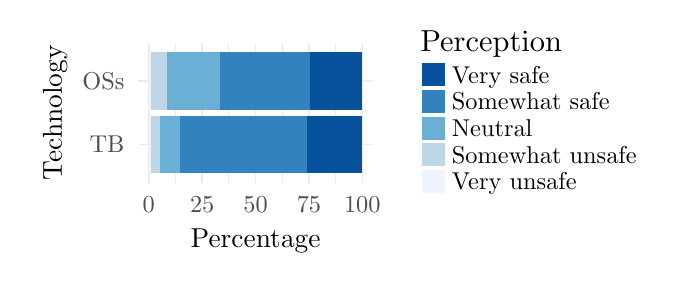
\begin{tikzpicture}[x=1pt,y=1pt]
\definecolor{fillColor}{RGB}{255,255,255}
\path[use as bounding box,fill=fillColor,fill opacity=0.00] (0,0) rectangle (231.26, 86.72);
\begin{scope}
\path[clip] ( 39.91, 30.77) rectangle (124.79, 81.22);
\definecolor{drawColor}{gray}{0.92}

\path[draw=drawColor,line width= 0.3pt,line join=round] ( 53.42, 30.77) --
	( 53.42, 81.22);

\path[draw=drawColor,line width= 0.3pt,line join=round] ( 72.71, 30.77) --
	( 72.71, 81.22);

\path[draw=drawColor,line width= 0.3pt,line join=round] ( 92.00, 30.77) --
	( 92.00, 81.22);

\path[draw=drawColor,line width= 0.3pt,line join=round] (111.29, 30.77) --
	(111.29, 81.22);

\path[draw=drawColor,line width= 0.6pt,line join=round] ( 39.91, 44.53) --
	(124.79, 44.53);

\path[draw=drawColor,line width= 0.6pt,line join=round] ( 39.91, 67.46) --
	(124.79, 67.46);

\path[draw=drawColor,line width= 0.6pt,line join=round] ( 43.77, 30.77) --
	( 43.77, 81.22);

\path[draw=drawColor,line width= 0.6pt,line join=round] ( 63.06, 30.77) --
	( 63.06, 81.22);

\path[draw=drawColor,line width= 0.6pt,line join=round] ( 82.35, 30.77) --
	( 82.35, 81.22);

\path[draw=drawColor,line width= 0.6pt,line join=round] (101.64, 30.77) --
	(101.64, 81.22);

\path[draw=drawColor,line width= 0.6pt,line join=round] (120.93, 30.77) --
	(120.93, 81.22);
\definecolor{fillColor}{RGB}{239,243,255}

\path[fill=fillColor] ( 43.77, 34.21) rectangle ( 44.51, 54.85);
\definecolor{fillColor}{RGB}{189,215,231}

\path[fill=fillColor] ( 44.51, 34.21) rectangle ( 47.92, 54.85);
\definecolor{fillColor}{RGB}{107,174,214}

\path[fill=fillColor] ( 47.92, 34.21) rectangle ( 54.90, 54.85);
\definecolor{fillColor}{RGB}{49,130,189}

\path[fill=fillColor] ( 54.90, 34.21) rectangle (100.90, 54.85);
\definecolor{fillColor}{RGB}{8,81,156}

\path[fill=fillColor] (100.90, 34.21) rectangle (120.93, 54.85);
\definecolor{fillColor}{RGB}{239,243,255}

\path[fill=fillColor] ( 43.77, 57.15) rectangle ( 44.67, 77.78);
\definecolor{fillColor}{RGB}{189,215,231}

\path[fill=fillColor] ( 44.67, 57.15) rectangle ( 50.19, 77.78);
\definecolor{fillColor}{RGB}{107,174,214}

\path[fill=fillColor] ( 50.19, 57.15) rectangle ( 69.60, 77.78);
\definecolor{fillColor}{RGB}{49,130,189}

\path[fill=fillColor] ( 69.60, 57.15) rectangle (101.98, 77.78);
\definecolor{fillColor}{RGB}{8,81,156}

\path[fill=fillColor] (101.98, 57.15) rectangle (120.93, 77.78);
\end{scope}
\begin{scope}
\path[clip] (  0.00,  0.00) rectangle (231.26, 86.72);
\definecolor{drawColor}{gray}{0.30}

\node[text=drawColor,anchor=base east,inner sep=0pt, outer sep=0pt, scale=  0.88] at ( 34.96, 41.50) {TB};

\node[text=drawColor,anchor=base east,inner sep=0pt, outer sep=0pt, scale=  0.88] at ( 34.96, 64.43) {OSs};
\end{scope}
\begin{scope}
\path[clip] (  0.00,  0.00) rectangle (231.26, 86.72);
\definecolor{drawColor}{gray}{0.30}

\node[text=drawColor,anchor=base,inner sep=0pt, outer sep=0pt, scale=  0.88] at ( 43.77, 19.76) {0};

\node[text=drawColor,anchor=base,inner sep=0pt, outer sep=0pt, scale=  0.88] at ( 63.06, 19.76) {25};

\node[text=drawColor,anchor=base,inner sep=0pt, outer sep=0pt, scale=  0.88] at ( 82.35, 19.76) {50};

\node[text=drawColor,anchor=base,inner sep=0pt, outer sep=0pt, scale=  0.88] at (101.64, 19.76) {75};

\node[text=drawColor,anchor=base,inner sep=0pt, outer sep=0pt, scale=  0.88] at (120.93, 19.76) {100};
\end{scope}
\begin{scope}
\path[clip] (  0.00,  0.00) rectangle (231.26, 86.72);
\definecolor{drawColor}{RGB}{0,0,0}

\node[text=drawColor,anchor=base,inner sep=0pt, outer sep=0pt, scale=  0.99] at ( 82.35,  7.44) {Percentage};
\end{scope}
\begin{scope}
\path[clip] (  0.00,  0.00) rectangle (231.26, 86.72);
\definecolor{drawColor}{RGB}{0,0,0}

\node[text=drawColor,rotate= 90.00,anchor=base,inner sep=0pt, outer sep=0pt, scale=  0.99] at ( 12.32, 56.00) {Technology};
\end{scope}
\begin{scope}
\path[clip] (  0.00,  0.00) rectangle (231.26, 86.72);
\definecolor{drawColor}{RGB}{0,0,0}

\node[text=drawColor,anchor=base west,inner sep=0pt, outer sep=0pt, scale=  1.10] at (141.86, 78.11) {Perception};
\end{scope}
\begin{scope}
\path[clip] (  0.00,  0.00) rectangle (231.26, 86.72);
\definecolor{fillColor}{RGB}{8,81,156}

\path[fill=fillColor] (142.58, 65.57) rectangle (150.79, 73.78);
\end{scope}
\begin{scope}
\path[clip] (  0.00,  0.00) rectangle (231.26, 86.72);
\definecolor{fillColor}{RGB}{49,130,189}

\path[fill=fillColor] (142.58, 55.93) rectangle (150.79, 64.15);
\end{scope}
\begin{scope}
\path[clip] (  0.00,  0.00) rectangle (231.26, 86.72);
\definecolor{fillColor}{RGB}{107,174,214}

\path[fill=fillColor] (142.58, 46.30) rectangle (150.79, 54.51);
\end{scope}
\begin{scope}
\path[clip] (  0.00,  0.00) rectangle (231.26, 86.72);
\definecolor{fillColor}{RGB}{189,215,231}

\path[fill=fillColor] (142.58, 36.66) rectangle (150.79, 44.87);
\end{scope}
\begin{scope}
\path[clip] (  0.00,  0.00) rectangle (231.26, 86.72);
\definecolor{fillColor}{RGB}{239,243,255}

\path[fill=fillColor] (142.58, 27.03) rectangle (150.79, 35.24);
\end{scope}
\begin{scope}
\path[clip] (  0.00,  0.00) rectangle (231.26, 86.72);
\definecolor{drawColor}{RGB}{0,0,0}

\node[text=drawColor,anchor=base west,inner sep=0pt, outer sep=0pt, scale=  0.88] at (153.31, 66.65) {Very safe};
\end{scope}
\begin{scope}
\path[clip] (  0.00,  0.00) rectangle (231.26, 86.72);
\definecolor{drawColor}{RGB}{0,0,0}

\node[text=drawColor,anchor=base west,inner sep=0pt, outer sep=0pt, scale=  0.88] at (153.31, 57.01) {Somewhat safe};
\end{scope}
\begin{scope}
\path[clip] (  0.00,  0.00) rectangle (231.26, 86.72);
\definecolor{drawColor}{RGB}{0,0,0}

\node[text=drawColor,anchor=base west,inner sep=0pt, outer sep=0pt, scale=  0.88] at (153.31, 47.37) {Neutral};
\end{scope}
\begin{scope}
\path[clip] (  0.00,  0.00) rectangle (231.26, 86.72);
\definecolor{drawColor}{RGB}{0,0,0}

\node[text=drawColor,anchor=base west,inner sep=0pt, outer sep=0pt, scale=  0.88] at (153.31, 37.74) {Somewhat unsafe};
\end{scope}
\begin{scope}
\path[clip] (  0.00,  0.00) rectangle (231.26, 86.72);
\definecolor{drawColor}{RGB}{0,0,0}

\node[text=drawColor,anchor=base west,inner sep=0pt, outer sep=0pt, scale=  0.88] at (153.31, 28.10) {Very unsafe};
\end{scope}
\end{tikzpicture}

    \caption{The level of security our respondents perceive when using Tor
    Browser (TB) and onion services (OSs).}
    \label{fig:perceived-security}
\end{figure}

Asked about why our respondents feel that way about Tor Browser, our results
reveal that non-experts lack the ability to evaluate (or even understand) Tor's
design which is why they defer to expert opinion, their gut feeling, or the
trust they have in Tor developers.  The Tor Project is perceived to take
security and privacy more seriously than any other browser vendor, which is
appreciated among our respondents.  Most of our respondents' criticism focused
not on Tor Browser but on the underlying Firefox code base.  Many participants
were unhappy with the exploit mitigation techniques, the lack of sandboxing, and
the complex code base.  Chrome was sometimes brought up as the golden standard
for browser security.\footnote{Note that our survey was run before Mozilla
released Firefox Quantum on Nov 14, 2017, which brought substantial improvements
in both security and usability.}  Malicious exit relays were a concern for a
handful of participants while another couple of participants are concerned that
their use of Tor makes them stick out and turn into a target for government
agencies.  Some participants weren't sure if their Tor setup works properly---a
common theme that we also noticed in our interviews: Non-technical users desire
visual feedback confirming that their network traffic comes out ``somewhere
else.''

With respect to onion services, the majority expressed that the added security
and anonymity makes them feel safe.  Another factor contributing to the
perceived security is that onion services make use of far fewer advertising
companies.  Orthogonal to the technology, many participants voiced concern about
illegal and questionable content on onion services, described by some as a
``Wild West.''  Phishing sites, honeypots, and compromised onion sites further
contribute to this perception.
